\subsection{Esperimento 2: valutazione del metodo di campionamento migliore}\label{subsec:exp2}
Una volta verificata l'efficacia dell'algoritmo di esplorazione si vuole capire quale, tra le varie tecniche di campionamento, permette di avere dei valori di RCR ed esplorazione migliori.
Data l'uniformità dei risultati precedenti, i seguenti esperimenti sono stati svolti in scenari in cui erano presenti le BS.

\begin{table}[p]
\centering
\begin{tabular}{|c|c|c|c|c|c|}
\hline
Esplorazione & Systematic & Local & Penalty & Ann.forward & Ann.reverse \\
\hline
Massima & 0.86 & 0.87 & 0.86 & 0.87 & 0.86 \\
Minima & 0.79 & 0.79 & 0.79 & 0.81 & 0.81 \\
Media & 0.83 & 0.84 & 0.82 & 0.85 & 0.84 \\
Dev. standard & 0.017 & 0.017 & 0.020 & 0.015 & 0.014 \\
\hline
\end{tabular}
\caption{\label{tab:exp2_expl_statistics}Secondo esperimento, indici dei valori finali di esplorazione.}

\vspace*{0.5 cm}

\begin{tabular}{|c|c|c|c|c|c|}
\hline
Copertura & Systematic & Local & Penalty & Ann.forward & Ann.reverse \\
\hline
Massima & 0.97 & 0.97 & 0.93 & 1 & 0.97 \\
Minima & 0.7 & 0.73 & 0.6 & 0.7 & 0.77 \\
Media & 0.83 & 0.86 & 0.82 & 0.86 & 0.88 \\
Dev. standard & 0.067 & 0.060 & 0.087 & 0.072 & 0.056 \\
\hline
\end{tabular}
\caption{\label{tab:exp2_cov_statistics}Secondo esperimento, indici dei valori finali di copertura.}

\vspace*{0.5 cm}

\begin{tabular}{|c|c|c|c|c|c|}
\hline
 & Systematic & Local & Penalty & Ann.forward & Ann.reverse \\
\hline
tempo medio & 849.3 & 384 & 835.3 & 515 & 495.1 \\
\hline
\end{tabular}
\caption{\label{tab:exp2_time comparison}
Secondo esperimento, tempi medi di esecuzione.}
\end{table}

\begin{figure}[p]
    \centering
    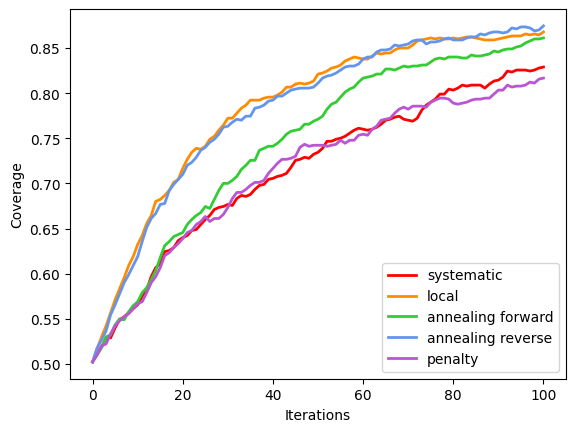
\includegraphics[width=0.8\textwidth]{img/ch4/experiment2/coverages_graphic_comparison.png}
    \caption[Grafici di copertura nel secondo esperimento]{Secondo esperimento, confronto tra i valori medi di copertura utente.}
    \label{fig:confronto_cov_exp2}

\vspace*{0.5cm}

    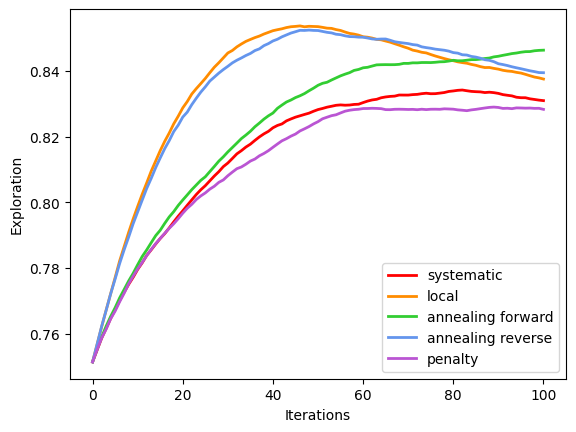
\includegraphics[width=0.8\textwidth]{img/ch4/experiment2/exploration_graphic_comparison.png}
    \caption[Grafici di esplorazione nel secondo esperimento]{Secondo esperimento, confronto dell'andamento medio di esplorazione tra le varie tecniche di campionamento.}
    \label{fig:confronto_expl_exp2}
\end{figure}

Osservando i valori di \textbf{esplorazione} (Figura \ref{fig:confronto_expl_exp2}), si constata che i metodi \textit{local} e \textit{annealing reverse} raggiungo dei livelli molto alti in breve tempo, per poi favorire le posizioni raggiunte dagli agenti.
La tecnica \textit{Annealing forward} invece, a fronte di un transitorio meno rapido, riesce a raggiungere valori finali più alti, come si vede anche in Tabella \ref{tab:exp2_expl_statistics}.
Analizzando i livelli di \textbf{copertura} (Figura \ref{fig:confronto_cov_exp2}), si nota come i metodi \textit{local} e \textit{annealing reverse} risultino i più performanti, sia per i livelli finali raggiunti (Tabella \ref{tab:exp2_cov_statistics}) sia per la velocità di convergenza.
Queste due tecniche sembrano quindi del tutto equivalenti; tuttavia analizzando i tempi di esecuzione in Tabella \ref{tab:exp2_time comparison} si osserva che il tempo della tecnica \textit{local} è circa del 28\% minore rispetto a quello della tecnica \textit{annealing reverse} , portando quindi a favorire la prima per la sua maggiore velocità di esecuzione.